\documentclass[conference]{IEEEtran}
\usepackage[T1]{fontenc}
\usepackage{amsmath,amssymb}
\usepackage{booktabs}
\usepackage{graphicx}
\usepackage{xcolor}
\usepackage{tikz}
\usetikzlibrary{arrows.meta,positioning,calc}
\usepackage{pgfplots}
\pgfplotsset{compat=1.18}
\usepackage{xurl}
\usepackage{draftwatermark}
\SetWatermarkText{PRELIMINARY DRAFT}
\SetWatermarkScale{0.55}
\SetWatermarkColor[gray]{0.92}

\newcommand{\sys}{\textsc{DeltaProof}}
\newtheorem{theorem}{Theorem}
\newtheorem{lemma}{Lemma}
\newtheorem{corollary}{Corollary}
\newtheorem{proposition}{Proposition}

\begin{document}

\title{Difference-Proportional Verification of Live Heterogeneous Database Migrations with Invertible Bloom Lookup Tables}

\author{\IEEEauthorblockN{Nithin Narla}
\IEEEauthorblockA{Independent Researcher\\
nithin.nnv@gmail.com}
\and
\IEEEauthorblockN{Suhas Jangoan}
\IEEEauthorblockA{suhas.jangoan@ieee.org}}

\maketitle

\begin{abstract}
Migrating a live system from one database to another, for example from a relational store to a wide-column NoSQL store, requires evidence that the two stores hold identical data. Existing tools compare full scans or checksum key ranges and bisect mismatches. Their cost grows with table size, they assume both stores scan in the same key order, and they report false differences while writes are in flight. We present \sys{}, a verifier whose communication cost grows with the number of differences rather than the size of the data. Each store maintains partitioned invertible Bloom lookup tables (IBLTs) over a canonical encoding of its records. Subtracting the two sketches and decoding the result yields the exact differing keys in one round, independent of key order. A watermark and confirmation protocol separates replication lag from true divergence, and a ladder of sketch sizes chosen by a strata estimator avoids decoding failures. On up to $10^7$ ledger entries with eight injected fault classes, \sys{} found every injected difference with no false positives. At $10^7$ rows and about 1{,}100 differences it transferred 0.78\,MB and read no table rows, while Merkle trees transferred 32\,MB, range-checksum bisection 280\,MB and a full scan 480\,MB, each reading 20--52 million rows. Between real PostgreSQL~16 and Cassandra~4.1 stores, \sys{} found all 120 injected faults; a digest without canonical encoding falsely flagged 99.9\% of rows. Under a live TPC-C workload replicated from PostgreSQL to Cassandra through a change stream, sketches maintained from the stream stayed exact, verification ran every 10\,s, version-aware confirmation made no false report in 38 checks, including with out-of-order replication, and the final answers were exact. Against PinSketch, \sys{} sends 3--9$\times$ more bytes but decodes 5--10$\times$ faster beyond $10^4$ differences and is cheaper to maintain per write.
\end{abstract}

\begin{IEEEkeywords}
data migration, set reconciliation, invertible Bloom lookup tables, data verification, heterogeneous databases, consistency
\end{IEEEkeywords}

\section{Introduction}
A live migration is complete only when the source and target stores provably hold the same data. For financial ledgers, payments and inventory, one missing or altered record is a correctness failure. Live migrations combine dual writes or change data capture (CDC), a backfill of historical data and a final cutover~\cite{xu2017,rae2013}. Verification is the weak step. Current practice falls into three groups:
\begin{itemize}
\item \emph{Full scans} read every record from both stores. Cost grows with table size and loads production databases.
\item \emph{Range-checksum bisection}~\cite{datadiff} hashes key ranges in both stores and splits mismatched ranges. It needs aligned key order, which hash-partitioned stores such as Cassandra~\cite{lakshman2010} do not provide, and several round trips.
\item \emph{Merkle-tree anti-entropy}~\cite{lakshman2010,merkle1987} compares replicas of one database with identical encodings and repairs whole segments.
\end{itemize}
None targets the common case of a heterogeneous migration: many records, few differences, different storage orders and encodings, and writes still arriving.

We observe that this is a \emph{set reconciliation} problem. IBLTs~\cite{goodrich2011,eppstein2011} reconcile sets with communication proportional to the size of the difference, in one round and independent of order. IBLTs are also linear, so sketches can be maintained from a change stream instead of rebuilt by scanning. We contribute:
\begin{enumerate}
\item a canonical record encoding that hashes logically equal records identically across relational and wide-column stores (Section~\ref{sec:canon});
\item partitioned, incrementally maintained IBLT sketches with a size ladder selected by a strata estimator (Section~\ref{sec:design});
\item a watermark and confirmation protocol for verification while writes are in flight (Section~\ref{sec:live});
\item an open-source implementation and an evaluation against full scans, bisection, Merkle trees, aggregates and PinSketch, in process up to $10^7$ rows, on TPC-H data, and under a live TPC-C workload replicated from PostgreSQL to Cassandra (Sections~\ref{sec:impl}--\ref{sec:eval}).
\end{enumerate}

\section{Background}
\subsection{Live migration model}
The source store $S$ stays authoritative. A dual-write or CDC path copies new writes to the target $T$ and a backfill copies history. Verification must show $S=T$ before reads and then writes move to $T$. Records have a primary key $k$, a value $v$ and a source commit version.

\subsection{Divergence classes}
Table~\ref{tab:faults} lists the faults a verifier must catch; each becomes an injected fault in Section~\ref{sec:eval}. Offsetting errors, such as one lost and one duplicated entry of equal amount, leave counts and sums unchanged and defeat aggregate checks.

\begin{table}[t]
\caption{Divergence classes and their effect on the target}
\label{tab:faults}
\centering\footnotesize
\begin{tabular}{@{}lll@{}}
\toprule
Fault & Example cause & Effect on $T$\\
\midrule
Lost write & Secondary write fails silently & Key missing\\
Phantom & Retry without idempotency & Extra key\\
Stale value & Backfill overwrites newer write & Old value\\
Corruption & Type-mapping bug & Wrong value\\
Precision & Decimal $\to$ float rounding & Amount off by 0.01\\
Time zone & Timestamp without zone & Time off by hours\\
Lost delete & Delete not propagated & Extra key\\
Offsetting & Lost write + equal phantom & Aggregates unchanged\\
\bottomrule
\end{tabular}
\end{table}

\subsection{Invertible Bloom lookup tables}
An IBLT~\cite{goodrich2011} is an array of $m$ cells; each element $x$ is hashed into $q$ cells (we use $q=3$ subtables). A cell holds a count, an XOR of keys and an XOR of checksums:
\begin{equation}
\mathrm{count} \mathrel{+}= 1,\quad \mathrm{keySum} \mathrel{\oplus}= h(x),\quad \mathrm{checkSum} \mathrel{\oplus}= g(x).
\end{equation}
Two sketches built with the same hashes subtract cell by cell; common elements cancel, leaving the symmetric difference. \emph{Peeling} recovers it: a cell with count $\pm1$ and a valid checksum holds one element, which is removed from its other cells. Decoding succeeds with high probability when $m$ exceeds about $1.23$ times the number of differences $d$ for $q=3$~\cite{goodrich2011,eppstein2011}. Strata estimators~\cite{eppstein2011} and rateless designs~\cite{yang2024} handle unknown $d$.

\section{\sys{} Design}\label{sec:design}
\begin{figure}[t]
\centering
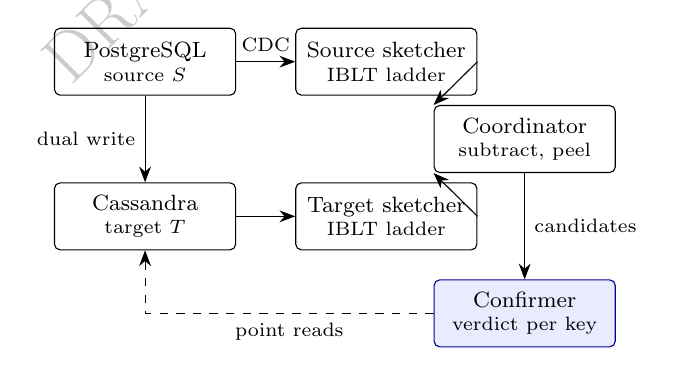
\begin{tikzpicture}[font=\footnotesize, box/.style={draw, rounded corners=2pt, minimum width=2.3cm, minimum height=0.85cm, align=center}, >={Stealth[length=2mm]}]
\node[box] (pg) {PostgreSQL\\[-1pt]\scriptsize source $S$};
\node[box, below=1.1cm of pg] (cs) {Cassandra\\[-1pt]\scriptsize target $T$};
\node[box, right=0.75cm of pg] (ss) {Source sketcher\\[-1pt]\scriptsize IBLT ladder};
\node[box, right=0.75cm of cs] (ts) {Target sketcher\\[-1pt]\scriptsize IBLT ladder};
\node[box, right=0.6cm of $(ss)!0.5!(ts)$] (co) {Coordinator\\[-1pt]\scriptsize subtract, peel};
\node[box, below=1.35cm of co, fill=blue!8, draw=blue!60!black] (cf) {Confirmer\\[-1pt]\scriptsize verdict per key};
\draw[->] (pg) -- node[left, font=\scriptsize] {dual write} (cs);
\draw[->] (pg) -- node[above, font=\scriptsize] {CDC} (ss);
\draw[->] (cs) -- (ts);
\draw[->] (ss.east) -- (co.north west);
\draw[->] (ts.east) -- (co.south west);
\draw[->] (co) -- node[right, font=\scriptsize] {candidates} (cf);
\draw[->, dashed] (cf.west) -| node[pos=0.25, below, font=\scriptsize] {point reads} (cs.south);
\end{tikzpicture}
\caption{\sys{} architecture. Only sketches cross between the stores; individual records are read only for candidate keys.}
\label{fig:arch}
\end{figure}

\subsection{Canonical record encoding}\label{sec:canon}
Each record becomes an element $e=(k,\delta)$ with a 128-bit key and a 64-bit digest $\delta = H_{64}(\mathrm{canon}(v))$ of the canonical value. The canonical form fixes the column order through the migration's schema mapping, and normalizes each type: decimals become exact scaled integers at a declared scale; timestamps become UTC at a declared unit (milliseconds when one store keeps only milliseconds); text is Unicode NFC; \texttt{CHAR($n$)} padding is dropped; floats are compared by IEEE-754 bits with $-0.0$ and NaN folded; nulls carry their own tag, so $\mathrm{null}\neq\texttt{""}\neq 0$. Composite keys of up to four integer parts are packed with an 8-bit table tag into 128 bits, so one sketch covers many tables. A changed value appears as two elements with the same key and is reported as a \emph{value mismatch}.

\subsection{Partitioned sketches and the size ladder}
Records are assigned to $P$ partitions by a hash of the key, independent of physical order. Each partition is an IBLT; a partition that fails to decode is the only one rescanned. Because update cost is linear, each store keeps a \emph{ladder} of levels at once, with capacities $C_i = 64\cdot 8^i$ up to $n/8$, $P_i=\max(1, C_i/256)$ partitions and $2C_i/P_i$ cells each. Verification sends a 32-stratum estimator first. If every stratum decodes, the difference is already exact; otherwise the coordinator decodes the smallest level with $C_i \geq 1.25\,\hat d$. Inserts add an element, deletes remove one, and updates remove the old element and add the new one, so sketches follow a change stream without rescans.

\section{Verifying While Writes Are In Flight}\label{sec:live}
During a live migration $T$ trails $S$ by the replication lag, so a naive comparison reports every in-flight write. \sys{} tags each sketch snapshot with a \emph{watermark}, the highest source commit version it reflects, and compares $S$ at the target's watermark $w$. Writes applied to $T$ out of order, ahead of $w$, still appear as candidates, so each candidate is \emph{confirmed} by re-reading both stores: equal values mean the write was in flight; if $T$ is behind, the key is re-checked after a grace period $\Delta$; a key that still differs is reported. Re-reads are point lookups on candidate keys only. In-flight writes enlarge the difference, so with write rate $\lambda$ and lag $L$ a level must hold about
\begin{equation}
m \approx c\cdot \frac{d_{\mathrm{true}} + \lambda L}{P},\qquad c\approx 2,
\end{equation}
cells per partition; the strata estimator measures this combined size directly.

Section~\ref{sec:proofs} proves when this protocol is exact and states precisely what confirmation guarantees.

\section{Correctness}\label{sec:proofs}
\subsection{Model}
Let $\mathcal K$ be the key space and $\mathcal U=\mathcal K\times\{0,1\}^{64}$ the element space. A store state is a partial map $\sigma:\mathcal K\rightharpoonup\mathcal V$; its element set is $E(\sigma)=\{(k,\delta(\sigma(k))) : k\in\mathrm{dom}\,\sigma\}$ with $\delta=H_{64}\circ\mathrm{canon}$. Two values are \emph{equivalent}, $v\equiv v'$, if $\mathrm{canon}(v)=\mathrm{canon}(v')$; this is the equality the schema mapping declares (Section~\ref{sec:canon}). We model $H_{64}$, the cell-placement hashes $h_1,\dots,h_q$ and the checksum $g$ as independent random functions (the random-oracle model), and write $\varepsilon=2^{-64}$.

A \emph{signed multiset} is $f:\mathcal U\to\mathbb Z$ with finite support. A sketch with $m$ cells is $\Phi(f)\in G^m$, $G=\mathbb Z\times\mathbb F_2^{128}\times\mathbb F_2^{64}\times\mathbb F_2^{64}$, where cell $c$ holds
\begin{align*}
\Big(&\textstyle\sum_{x\in c} f(x),\ \bigoplus_{x\in c} [f(x)]_2\, k(x),\\
&\textstyle\bigoplus_{x\in c}[f(x)]_2\,\delta(x),\ \bigoplus_{x\in c}[f(x)]_2\, g(x)\Big),
\end{align*}
``$x\in c$'' means $h_j(x)=c$ for some $j$ (the $q$ subtables make the $q$ cells of $x$ distinct), and $[\cdot]_2$ is reduction mod~2. We write $\mathbf 1_A$ for the indicator of a set $A$.

\subsection{Sketches follow the data}
\begin{lemma}[Linearity]\label{lem:lin}
$\Phi(f+f')=\Phi(f)\boxplus\Phi(f')$, where $\boxplus$ adds counts and XORs the other fields.
\end{lemma}
\begin{IEEEproof}
Each field of each cell is the image of $f$ under a group homomorphism: summation into $\mathbb Z$ for the count, and $f\mapsto\bigoplus [f(x)]_2\,a(x)$ for the others, because $[\cdot]_2:\mathbb Z\to\mathbb F_2$ is a homomorphism. A sum of homomorphisms is a homomorphism.
\end{IEEEproof}

\begin{lemma}[Change-stream maintenance]\label{lem:stream}
Let $\sigma_0$ be the state at which the sketch is built and $c_1,c_2,\dots$ the changes after it in commit order, where $c_i$ on key $k_i$ carries a before-image $b_i$ and an after-image $a_i$ (either may be absent). If every before-image is complete, $b_i=\sigma_{i-1}(k_i)$, then applying $-\mathbf 1_{e(b_i)}+\mathbf 1_{e(a_i)}$ for $i\le r$ to $\Phi(\mathbf 1_{E(\sigma_0)})$ yields $\Phi(\mathbf 1_{E(\sigma_r)})$, where $e(\cdot)$ is the element of a row and $e(\text{absent})$ contributes nothing.
\end{lemma}
\begin{IEEEproof}
Only key $k_i$ changes at step $i$, so $\mathbf 1_{E(\sigma_i)}=\mathbf 1_{E(\sigma_{i-1})}-\mathbf 1_{e(b_i)}+\mathbf 1_{e(a_i)}$ because $b_i=\sigma_{i-1}(k_i)$. Induct on $i$ and apply Lemma~\ref{lem:lin}.
\end{IEEEproof}

In PostgreSQL, \texttt{REPLICA IDENTITY FULL} makes before-images complete. The same lemma covers the target sketch when its before-images come from the side table of last written digests, provided nothing writes to the target outside the pipeline.

\subsection{Decoding is exact or reports failure}
For states $S,T$ let $\Delta=\mathbf 1_{E(S)}-\mathbf 1_{E(T)}$; then $\Delta(x)\in\{-1,0,1\}$, and by Lemma~\ref{lem:lin} the subtracted sketch is $\Phi(\Delta)$. Peeling accepts a cell when its count is $\pm1$ and its checksum equals $g(x^\ast)$ for the element $x^\ast$ formed by its key and digest fields; it then subtracts $\pm\mathbf 1_{\{x^\ast\}}$. It reports success when no cell is left nonzero.

\begin{theorem}[Exact decoding]\label{thm:decode}
Let peeling of $\Phi(\Delta)$ examine $N$ cells and output $O$. If it reports success, then $O=\Delta$ except with probability at most $(N+1)\varepsilon$. If it reports failure, the nonzero cells identify every partition whose elements may be incomplete.
\end{theorem}
\begin{IEEEproof}
Call an acceptance \emph{false} if the accepted cell's residual content $R=\mathrm{supp}(\Delta-O)\cap c$ is not exactly $\{x^\ast\}$. Until the first false acceptance, the invariant ``the table equals $\Phi(\Delta-O)$ and $O$ agrees with $\Delta$ on $\mathrm{supp}\,O$'' holds, because a truly pure cell yields $x^\ast\in\mathrm{supp}\,\Delta$ with the right sign. Before the first false acceptance, which cells are examined and in what order depends only on $\Delta$ and the placement hashes, so it is independent of $g$. A false acceptance at a cell needs $\bigoplus_{y\in R}g(y)=g(x^\ast)$ with $R\neq\{x^\ast\}$ and $R\neq\emptyset$ (an empty $R$ has count $0$). If $x^\ast\notin R$, then $g(x^\ast)$ is independent of $\{g(y)\}_{y\in R}$; otherwise $\bigoplus_{y\in R\setminus\{x^\ast\}}g(y)=0$ for a nonempty set. Either way the probability is $\varepsilon$, and a union bound over the $N$ examinations gives $N\varepsilon$. If peeling reports success but $\Delta'=\Delta-O\neq0$, pick $x\in\mathrm{supp}\,\Delta'$ and a cell $c\ni x$: its checksum field $\bigoplus_{y\in R_c}g(y)$ is $0$ with $x\in R_c$, which has probability $\varepsilon$. This adds the final $\varepsilon$. Cells are zero only when every partition decoded, so the nonzero cells name every incomplete partition.
\end{IEEEproof}

\begin{corollary}[Correctness independent of sizing]\label{cor:exact}
Let $D(S,T)=\{k: S(k)\not\equiv T(k)\}$, where an absent key is equivalent only to an absent key. Verification returns $D(S,T)$, split into missing, extra and mismatched keys, except with probability at most $(N+1)\varepsilon+|D(S,T)|\varepsilon$, for any choice of level, partition count or estimate.
\end{corollary}
\begin{IEEEproof}
Partitions that decode contribute exactly their part of $\mathrm{supp}\,\Delta$ by Theorem~\ref{thm:decode}; failed partitions are compared exactly by rescanning. Each store contributes at most one element per key, so for each key $\mathrm{supp}\,\Delta$ holds nothing, one element of either sign, or one of each sign with different digests; these are exactly ``equal'', ``missing in $T$'', ``extra in $T$'' and ``value mismatch''. A key with $S(k)\not\equiv T(k)$ is missed only if $H_{64}$ maps the two different canonical values to the same digest, which happens with probability $\varepsilon$ per such key.
\end{IEEEproof}

The strata estimate and the ladder level therefore affect cost, not correctness. The canonical words are bijections of the canonical values (SplitMix64 is invertible), so collisions arise only in $H_{64}$ and in the 64-bit text hash, both covered by $\varepsilon$ in the random-oracle model.

\subsection{Verification while writes are in flight}
Let source changes have versions in commit order, and let $S_w$ be the source state after all changes with version $\le w$. The replicator \emph{processes} each change: it applies it, applies it altered, or drops it. Its \emph{watermark} $w_T$ is the largest $w$ such that every change with version $\le w$ has been processed.

\begin{theorem}[Watermark exactness]\label{thm:wm}
Assume Lemma~\ref{lem:stream}'s conditions on both sides and \emph{in-order application}: at the verification instant the target reflects the processing of exactly the changes with version $\le w_T$. Then verification of $\Phi(\mathbf 1_{E(S_{w_T})})$ against the target sketch returns $D(S_{w_T},T)$, the keys on which the pipeline's processing of the first $w_T$ changes diverged, with the error bound of Corollary~\ref{cor:exact}. No confirmation is needed.
\end{theorem}
\begin{IEEEproof}
By Lemma~\ref{lem:stream} the source sketch advanced to $w_T$ is $\Phi(\mathbf 1_{E(S_{w_T})})$, and the target sketch is $\Phi(\mathbf 1_{E(T)})$ for the target's actual state. Apply Corollary~\ref{cor:exact} to $(S_{w_T},T)$.
\end{IEEEproof}

Our replicator satisfies in-order application: each batch is applied whole, with the sketch lock held, and verification runs between batches. Rescanned partitions compare current states rather than states at $w_T$, so their keys are candidates that need confirmation.

\begin{proposition}[Out-of-order application]\label{prop:ooo}
If the target reflects all changes with version $\le w_T$ plus a set $A$ of later changes, then the output $C$ satisfies $D(S_{w_T},T)\setminus\mathrm{keys}(A)\subseteq C\subseteq D(S_{w_T},T)\cup\mathrm{keys}(A)$.
\end{proposition}
\begin{IEEEproof}
For $k\notin\mathrm{keys}(A)$ the target value is that of in-order processing, so Theorem~\ref{thm:wm}'s argument applies key by key; keys in $\mathrm{keys}(A)$ may land on either side.
\end{IEEEproof}

\emph{Version-aware confirmation.} Let each target row record the source version $v_T(k)$ of the change that wrote it. From the change stream, keep for each key $k$ its state at the watermark, $(\lambda_w(k),\delta_w(k))$: the version of the last change to $k$ with version $\le w_T$ (0 if none since the sketch was built) and the digest after it, or ``absent''. Also keep the list $\Lambda(k)$ of pairs $(v,\delta_v)$ for delivered changes to $k$ with $v>w_T$. Let $V(k)=\{(\lambda_w(k),\delta_w(k))\}\cup\Lambda(k)$, the states the source held for $k$ at or after $w_T$. Report a candidate $k$ if and only if
\[
\big(v_T(k),\,\delta(T(k))\big)\notin V(k),
\]
where an absent target row matches any element of $V(k)$ whose digest is ``absent''. The rule reads only the target and the stream-fed index, never the source, and decides at once.

\begin{theorem}[Sound and complete confirmation]\label{thm:confirm}
Assume the target is written only by the pipeline. Up to $H_{64}$ collisions: (i) if $k$ is reported, the target holds for $k$ no state that the source held at or after $w_T$; (ii) if the pipeline's last processed change to $k$ has version at most $w_T$ and was processed incorrectly (dropped, altered, or applied over a newer state), then $k$ is reported.
\end{theorem}
\begin{IEEEproof}
(i) $(\lambda_w(k),\delta_w(k))$ is $k$'s source state at version $w_T$, and each $(v,\delta_v)\in\Lambda(k)$ is its state just after change $v>w_T$. So $V(k)$ contains only states the source held at or after $w_T$, and a target pair outside it matches none of them.
(ii) Let the faulty change $c$ have version $v_c\le w_T$, with no later change to $k$ processed. Then $\lambda_w(k)\ge v_c$ and every pair in $\Lambda(k)$ has version $>w_T\ge v_c$. If $c$ was dropped, or a stale state was written over it, the target holds a state written by an earlier change, with version $v'<v_c\le\lambda_w(k)$; a deleted key whose delete was dropped still holds such a row. That version is in no pair of $V(k)$. If $c$ was altered, the target holds $(v_c,\delta')$ with $\delta'\neq\delta_c$; when $v_c=\lambda_w(k)$ the digest differs from $\delta_w(k)$, and when $v_c<\lambda_w(k)$ the version matches no pair. In every case the target pair is not in $V(k)$, unless $H_{64}$ collides ($\varepsilon$).
\end{IEEEproof}

A fault on a change with version above $w_T$ may still match $(\lambda_w,\delta_w)$, so it is decided at a later check, once $w_T$ passes it. The sketch comparison supplies the candidates: under in-order application they are exactly the divergent keys (Theorem~\ref{thm:wm}), and under out-of-order application a superset (Proposition~\ref{prop:ooo}), which the rule filters.

\emph{Current-read confirmation.} A simpler rule needs no versions: re-read both stores at $t_1$ and again at $t_2\ge t_1+\Delta$, and report $k$ if both reads differ.

\begin{proposition}\label{prop:quiet}
If every change is processed within time $L<\Delta$ of its commit, and no change to $k$ commits in $[t_1-L,\,t_2]$, then current-read confirmation reports $k$ if and only if the pipeline processed $k$'s last change incorrectly.
\end{proposition}
\begin{IEEEproof}
The last change to $k$ committed before $t_1-L$, so it was processed by $t_1\le t_2$. No newer change exists by $t_2$, so $S(k)$ at $t_2$ is that change's after-image, and $T(k)$ at $t_2$ is its processed result. Both reads therefore differ exactly when the processing was incorrect.
\end{IEEEproof}

For keys written continually during the check, such as TPC-C's \texttt{district} rows, both reads can differ because of lag alone, so current-read confirmation can report a key that is only behind. The version-aware rule of Theorem~\ref{thm:confirm} removes this case, and our live experiments use it.

\section{Implementation}\label{sec:impl}
\sys{} is implemented in Python~3 with NumPy, about 1{,}100 lines for the library plus tests, benchmarks and adapters, released under the Apache~2.0 license [repository URL to be added]. Cells are 36 bytes on the wire (4-byte count, 16-byte key sum, 8-byte digest sum, 8-byte checksum). Hashing uses SplitMix64 mixing in bit-identical vectorized and scalar forms, and BLAKE2b-64 for text. The baselines share the encoder and a common cost model: bytes sent to the verifier, sequential round trips, and rows the stores read in bulk. Bisection is charged as if both stores could serve key-range checksums, its best case. Adapters read PostgreSQL through psycopg~3 and Cassandra through the DataStax driver.

\section{Evaluation}\label{sec:eval}
\subsection{Setup}
In-process experiments hold source and target as columnar arrays so that every method is measured under one cost model, with $n\in\{10^5,10^6,10^7\}$ entries of a synthetic double-entry ledger (Zipf-distributed accounts, $\theta=0.99$; log-normal amounts in cents; five currencies) and $d$ up to 112{,}500 differing keys. The end-to-end experiments use PostgreSQL~16.4 and Cassandra~4.1.6, single nodes in Docker, with the ledger, TPC-H \texttt{lineitem} and a live TPC-C workload. All runs used one Apple M1 Pro laptop (10 cores, 16\,GB), Python~3.13 and NumPy~2.5, seed 42.

\subsection{Detection (RQ1)}
Each fault class was injected alone, 100 faults into $10^6$ rows. \sys{}, the full scan, bisection and Merkle trees found 100\% of every class with no false positives. Per-partition count and sum aggregates detected lost writes, phantoms, stale values and lost deletes, but 84\% of precision faults and none of the corruption, time-zone or offsetting faults.

\subsection{Cost (RQ2)}
Every method returned exactly the injected keys in all 14 configurations. Fig.~\ref{fig:bytes} and Table~\ref{tab:cost} show the results at $n=10^7$. \sys{} read no table rows at verification time, while every baseline read about $2n$ rows or more. With no differences, Merkle trees (16\,B) and bisection (1\,KB) send less than \sys{}'s 187\,KB estimator, but only after scanning both tables. Near 1\% differing rows the advantage over a full scan shrinks to $12\times$.

\emph{PinSketch.} We also compared PinSketch, BCH-syndrome reconciliation~\cite{minsky2003,dodis2008}, using the minisketch C++ library~\cite{minisketch}. To be fair to it, PinSketch received \sys{}'s strata estimate and the same key partitioning, with each partition's capacity set to its expected load plus four standard deviations. It was exact in every configuration and is the stronger method on bandwidth: from 1{,}125 differences up, it sent $3.4$--$9.4\times$ fewer bytes than \sys{} (Table~\ref{tab:pinsketch}), because a 64-bit syndrome per unit of capacity is smaller than a 36-byte IBLT cell at load~0.5. \sys{} is the stronger method on computation. From 11{,}250 differences up it decoded $5$--$10\times$ faster (below that PinSketch decoded faster, as its $O(c^2)$ decoding is cheap at small capacity), and its whole ladder of six sizes was built for both stores in 18\,s, in NumPy, while one PinSketch sized for a known estimate took 34--37\,s in C++. Adding an element costs $q=3$ cell updates per IBLT level but one update per unit of capacity in a PinSketch partition, which matters when sketches follow every write of a change stream. The encoding, partitioning, watermark and confirmation in this paper apply to either sketch; IBLTs suit high write rates and PinSketch suits constrained links.

\begin{table}[t]
\caption{\sys{} vs.\ PinSketch at $n=10^7$}
\label{tab:pinsketch}
\centering\footnotesize
\setlength{\tabcolsep}{3pt}
\begin{tabular}{@{}rrrrrr@{}}
\toprule
& \multicolumn{2}{c}{MB sent} & \multicolumn{2}{c}{Decode (s)} & PinSketch\\
\cmidrule(lr){2-3}\cmidrule(lr){4-5}
$d$ & \sys{} & PinSketch & \sys{} & PinSketch & build (s)\\
\midrule
11 & 0.19 & 0.19 & 0.13 & 0.01 & 6.2\\
1{,}125 & 0.78 & 0.23 & 0.24 & 0.15 & 34.2\\
11{,}250 & 4.91 & 0.59 & 0.28 & 1.55 & 37.4\\
112{,}500 & 39.4 & 4.18 & 1.41 & 14.5 & 36.1\\
\bottomrule
\end{tabular}
\\[2pt]{\scriptsize \sys{}'s ladder, built once for any $d$, took 18--20\,s for both stores.}
\end{table}

\begin{figure}[t]
\centering
\begin{tikzpicture}
\begin{axis}[width=\columnwidth, height=5.4cm, xmode=log, ymode=log, xlabel={Differing keys}, ylabel={MB sent to verifier},
  legend style={font=\scriptsize, at={(0.5,-0.3)}, anchor=north, legend columns=2}, tick label style={font=\scriptsize}, label style={font=\footnotesize},
  ymin=0.1, ymax=1500, grid=major, grid style={gray!20}]
\addplot[blue!70!black, very thick, mark=*] table[x=d, y=deltaproof_mb] {data/rq2_n10000000.dat};
\addplot[orange!80!black, thick, mark=o] table[x=d, y=pinsketch_mb] {data/rq2_n10000000.dat};
\addplot[gray, mark=square*] table[x=d, y=merkle_mb] {data/rq2_n10000000.dat};
\addplot[gray!70, mark=triangle*] table[x=d, y=bisection_mb] {data/rq2_n10000000.dat};
\addplot[gray!50, mark=diamond*, dashed] table[x=d, y=full_scan_mb] {data/rq2_n10000000.dat};
\legend{\sys{}, PinSketch, Merkle tree, Range bisection, Full scan}
\end{axis}
\end{tikzpicture}
\caption{Bytes sent to the verifier at $n=10^7$ (log--log). \sys{}'s traffic grows with the number of differences; the baselines approach a full scan.}
\label{fig:bytes}
\end{figure}

\begin{table}[t]
\caption{Verification cost at $n=10^7$: MB sent / million rows read / round trips}
\label{tab:cost}
\centering\footnotesize
\setlength{\tabcolsep}{2.4pt}
\begin{tabular}{@{}rcccc@{}}
\toprule
$d$ & \sys{} & Merkle & Bisection & Full scan\\
\midrule
0 & 0.19 / 0 / 1 & 0.00 / 20.0 / 1 & 0.00 / 20.0 / 2 & 480 / 20.0 / 1\\
11 & 0.19 / 0 / 1 & 0.33 / 20.0 / 16 & 4.65 / 25.8 / 3 & 480 / 20.0 / 1\\
1{,}125 & 0.78 / 0 / 2 & 32.0 / 21.3 / 16 & 280 / 51.7 / 3 & 480 / 20.0 / 1\\
11{,}250 & 4.91 / 0 / 2 & 238 / 29.9 / 16 & 480 / 60.0 / 3 & 480 / 20.0 / 1\\
112{,}500 & 39.4 / 0.06 / 3 & 480 / 40.0 / 16 & 480 / 60.0 / 3 & 480 / 20.0 / 1\\
\bottomrule
\end{tabular}
\end{table}

\subsection{Live writes (RQ3)}
On $10^6$ rows with 50 true faults and 50{,}000 in-flight writes (Table~\ref{tab:live}), the naive comparison reported up to 9{,}942 false candidates. Watermarks alone removed them all when the target applied writes in order, but not when 10--50\% of later writes arrived early. With confirmation, every configuration reported exactly the 50 true faults and none falsely, at about two point reads per candidate.

\begin{table}[t]
\caption{False candidates under in-flight writes ($n=10^6$, 50 true faults)}
\label{tab:live}
\centering\small
\begin{tabular}{@{}rrrrrr@{}}
\toprule
Lag & Early & Naive & Watermark & +Confirm & Reads\\
\midrule
100 & 0\% & 100 & 0 & 0 & 100\\
1{,}000 & 10\% & 882 & 118 & 0 & 336\\
10{,}000 & 0\% & 9{,}942 & 0 & 0 & 100\\
10{,}000 & 50\% & 4{,}890 & 5{,}071 & 0 & 10{,}280\\
\bottomrule
\end{tabular}
\end{table}

\subsection{Overhead (RQ4) and robustness (RQ5)}
At $n=10^7$ the sketches took 173\,MB per store (17.3 bytes per row across six levels). Bulk loading cost 0.89\,\textmu s per row; batched updates of 2{,}000 writes cost 3.8\,\textmu s per write; single updates cost about 1.1\,ms, almost all Python interpreter overhead. A partition sized for 256 differences in 513 cells failed to decode in 0.3\% of trials at full load, 1.3\% at $1.25\times$, 10\% at $1.5\times$ and always at $2\times$. Strata estimates had median ratios of 0.98--1.00 to the true difference, with 90\% of estimates between 0.81 and 1.17, which supports the $1.25\times$ headroom. When a partition did fail, rescanning it cost at most 58{,}510 rows, 0.3\% of the rows in both stores.

\subsection{Real stores}
We loaded 200{,}000 entries into PostgreSQL and Cassandra and injected 120 faults of six classes with SQL and CQL statements. Scanning took 0.47\,s on PostgreSQL and 3.6\,s on Cassandra; canonical encoding took 4.3\,s and verification 12\,ms. \sys{} found all 120 faults with no false positives in two round trips and 260\,KB. A digest of the drivers' raw values flagged 199{,}835 rows, 199{,}715 of them falsely, because the stores format and round timestamps differently.

\subsection{TPC-H data}
To test the encoding on a standard schema we did not design, we generated TPC-H \texttt{lineitem} at scale factor 1 (6{,}001{,}215 rows) with \texttt{dbgen} through DuckDB, loaded it into PostgreSQL and Cassandra, and injected 120 faults of six classes (lost writes, precision, date shifts, corruption, lost deletes, phantoms). These are not TPC-H benchmark results. The exact difference of full scans of both stores equalled the injected set, and \sys{} found all 120 keys with no false positives in two round trips and 260\,KB; verification took 0.13\,s and building both sketches 11\,s. A digest of the drivers' raw values flagged every row, because PostgreSQL returns \texttt{CHAR($n$)} values padded and Cassandra's driver returns its own date type. Loading Cassandra took 750\,s and scanning with row-by-row canonical encoding took 222\,s on PostgreSQL and 397\,s on Cassandra in Python; a sketch fed by a change stream avoids these scans.

\subsection{Live TPC-C migration}
We ran BenchBase~\cite{difallah2013} TPC-C (4 warehouses, 8 terminals) on PostgreSQL. The eight TPC-C tables with primary keys hold 1.98 million rows; \texttt{history} has no key and is excluded. Changes were read with the wal2json logical-decoding plugin~\cite{wal2json}, with full before-images. A replicator applied them to Cassandra after a fixed lag, recorded the source version in each row, and dropped 0.05\% and corrupted 0.05\% of changes. In the out-of-order run it also deferred 5\% of changes by 0.5--1.5\,s, keeping per-key order, so later changes to other keys landed first. The source sketch followed the change stream, and the target sketch followed the values the replicator wrote. Every 10\,s, with the replicator paused between batches, \sys{} compared the sketches at the target's watermark and confirmed candidates with Theorem~\ref{thm:confirm}'s rule, which reads only the target. Each report was checked against what the replicator had actually done to that key's last processed change. At the end, both sketches were compared with sketches rebuilt from full scans, and the final answer with the exact difference of those scans.

\begin{table}[t]
\caption{Live TPC-C migration, PostgreSQL $\to$ Cassandra}
\label{tab:tpcc}
\centering\footnotesize
\setlength{\tabcolsep}{2.2pt}
\begin{tabular}{@{}lrrrr@{}}
\toprule
Rate (tx/s) & 200 & 200 & 200 & max\\
Lag; order & 2\,s & 5\,s & 2\,s; 5\% late & 2\,s\\
\midrule
Changes captured & 359{,}083 & 358{,}665 & 364{,}449 & 1{,}569{,}177\\
Injected faults & 330 & 332 & 344 & 1{,}510\\
Live checks & 11 & 11 & 10 & 6\\
Candidates (sum) & 1{,}500 & 1{,}528 & 40{,}622 & 813\\
Reported (sum) & 1{,}500 & 1{,}528 & 1{,}380 & 581\\
False reports / missed & 0 / 0 & 0 / 0 & 0 / 0 & 0 / 0\\
Median check time & 0.37\,s & 0.43\,s & 1.85\,s & 1.38\,s\\
True differences at end & 248 & 266 & 275 & 988\\
Final answer exact & yes & yes & yes & yes\\
Sketches equal rebuilds & yes & yes & yes & yes\\
\midrule
TPC-C p99, alone & 7.3\,ms & 7.3\,ms & 7.3\,ms & 9.2\,ms\\
TPC-C p99, with pipeline & 19.9\,ms & 18.1\,ms & 22.0\,ms & 17.3\,ms\\
TPC-C tx/s, alone / with & 200 / 200 & 200 / 200 & 200 / 200 & 3{,}368 / 1{,}963\\
\bottomrule
\end{tabular}
\end{table}

Table~\ref{tab:tpcc} summarizes four runs. Across 38 live checks no report was false and no fault on a change at or below the watermark was missed. With in-order application the candidates equalled the reports at every check, as Theorem~\ref{thm:wm} predicts. With 5\% of changes late, there were 27 times as many candidates as in the in-order run, as Proposition~\ref{prop:ooo} allows, and the version-aware rule removed every in-flight key. In the unlimited-rate run the replicator's 99th-percentile apply delay reached 147\,s with up to 610{,}000 queued changes, and verification stayed exact. In every run the sketches maintained from the change stream equalled full-scan rebuilds bit for bit, and the final answer equalled the true difference. Checks sent 187--778\,KB with in-order application and up to 4.9\,MB in the out-of-order run, whose in-flight keys enlarge the difference the sketches must hold (Section~\ref{sec:live}).

TPC-C's p99 latency at 200\,tx/s rose from 7.3\,ms alone to 18--22\,ms with the pipeline running; an earlier run of the same configuration measured 7.9\,ms. At an unlimited rate throughput fell 42\%. All components shared one 10-core laptop, so these numbers mix the cost of logical decoding with CPU contention from the Python replicator, Cassandra and BenchBase, and we treat them as upper bounds. Sketch maintenance, including canonical encoding, cost 39--42\,\textmu s per captured change and 37--44\,\textmu s per applied write in Python.

\section{Discussion and Limitations}
With no differences, the 187\,KB estimator costs more than a single root-hash comparison; a first round of one digest per store would close the gap. The live experiment ran every component on one laptop, so its source-overhead numbers at high load are an upper bound; separating the replicator onto its own machine is future work. The target sketch was maintained from the values the replicator wrote, so changes made to the target outside the pipeline would need the target's own change stream or periodic partition rescans to be seen. Single updates in Python are slow; batching change events reduces the cost to microseconds. Real-store tests used up to 6 million rows on single nodes. Tables without a primary key cannot be verified key by key. A wrong schema mapping could hide a mismatch if both sides are mis-encoded the same way, so mappings need their own tests.

\section{Related Work}
\emph{Set reconciliation.} Minsky \emph{et al.}~\cite{minsky2003} reconcile sets with near-optimal communication using characteristic polynomials, and PinSketch~\cite{dodis2008}, implemented in minisketch~\cite{minisketch}, does so with BCH syndromes; we compare against it in Section~\ref{sec:eval}; IBLTs~\cite{goodrich2011} with strata estimators~\cite{eppstein2011} made it practical, and rateless designs~\cite{yang2024} remove the need to estimate $d$. These target network synchronization; we add cross-store canonical encoding, CDC-fed maintenance and verification under live writes. \emph{Replica anti-entropy.} Cassandra repairs replicas with Merkle trees~\cite{lakshman2010,merkle1987}; practitioners have suggested IBLTs could improve full-table repair~\cite{scylla2026}. \emph{Migration verification.} data-diff~\cite{datadiff} bisects key-range checksums across databases. \emph{Online migration.} F1's online schema change~\cite{rae2013} and industry reports on dual writes~\cite{xu2017} address how to migrate, not how to prove the result; Kleppmann~\cite{kleppmann2017} surveys derived data and Helland~\cite{helland2007} motivates idempotent, entity-scoped processing.

\section{Conclusion}
Verifying a live heterogeneous migration is a set reconciliation problem. Treating it that way makes verification cost follow the number of differences instead of the data size. At $10^7$ rows and about 1{,}100 differences, \sys{} sent $41\times$ fewer bytes than the next-best method while reading no table rows, and it found every injected fault, with none reported falsely, on real PostgreSQL and Cassandra stores.

\section*{Acknowledgment}
During the preparation of this manuscript the authors used Claude (Anthropic) to assist with drafting and editing the text of all sections, writing the prototype implementation and benchmark scripts, and producing the figures and tables. All experiments were executed by running that code; every reported number comes from the resulting CSV files. The authors reviewed and take full responsibility for all content, including the verification of every citation.

\begin{thebibliography}{99}
\bibitem{xu2017} J.~Xu, ``Online migrations at scale,'' Stripe Engineering Blog, Feb. 2017. [Online]. Available: \url{https://stripe.com/blog/online-migrations}
\bibitem{rae2013} I.~Rae \emph{et al.}, ``Online, asynchronous schema change in F1,'' \emph{Proc. VLDB Endow.}, vol.~6, no.~11, pp.~1045--1056, 2013.
\bibitem{datadiff} data-diff, ``Technical explanation,'' project documentation. [Online]. Available: \url{https://data-diff.readthedocs.io/en/latest/technical-explanation.html}
\bibitem{lakshman2010} A.~Lakshman and P.~Malik, ``Cassandra: A decentralized structured storage system,'' \emph{ACM SIGOPS Oper. Syst. Rev.}, vol.~44, no.~2, pp.~35--40, 2010.
\bibitem{merkle1987} R.~C. Merkle, ``A digital signature based on a conventional encryption function,'' in \emph{Advances in Cryptology---CRYPTO '87}, LNCS vol.~293, 1988, pp.~369--378.
\bibitem{goodrich2011} M.~T. Goodrich and M.~Mitzenmacher, ``Invertible Bloom lookup tables,'' in \emph{Proc. 49th Annu. Allerton Conf. Commun., Control, Comput.}, 2011, pp.~792--799.
\bibitem{eppstein2011} D.~Eppstein, M.~T. Goodrich, F.~Uyeda, and G.~Varghese, ``What's the difference? Efficient set reconciliation without prior context,'' in \emph{Proc. ACM SIGCOMM}, 2011, pp.~218--229.
\bibitem{yang2024} L.~Yang, Y.~Gilad, and M.~Alizadeh, ``Practical rateless set reconciliation,'' in \emph{Proc. ACM SIGCOMM}, 2024.
\bibitem{dodis2008} Y.~Dodis, R.~Ostrovsky, L.~Reyzin, and A.~Smith, ``Fuzzy extractors: How to generate strong keys from biometrics and other noisy data,'' \emph{SIAM J. Comput.}, vol.~38, no.~1, pp.~97--139, 2008.
\bibitem{minisketch} P.~Wuille, G.~Maxwell, and G.~Naumenko, ``minisketch: An optimized library for BCH-based set reconciliation,'' GitHub repository. [Online]. Available: \url{https://github.com/bitcoin-core/minisketch}
\bibitem{minsky2003} Y.~Minsky, A.~Trachtenberg, and R.~Zippel, ``Set reconciliation with nearly optimal communication complexity,'' \emph{IEEE Trans. Inf. Theory}, vol.~49, no.~9, pp.~2213--2218, 2003.
\bibitem{kleppmann2017} M.~Kleppmann, \emph{Designing Data-Intensive Applications}. Sebastopol, CA, USA: O'Reilly Media, 2017.
\bibitem{helland2007} P.~Helland, ``Life beyond distributed transactions: An apostate's opinion,'' in \emph{Proc. CIDR}, 2007, pp.~132--141.
\bibitem{difallah2013} D.~E. Difallah, A.~Pavlo, C.~Curino, and P.~Cudr\'e-Mauroux, ``OLTP-Bench: An extensible testbed for benchmarking relational databases,'' \emph{Proc. VLDB Endow.}, vol.~7, no.~4, pp.~277--288, 2013.
\bibitem{wal2json} E.~Taveira, ``wal2json: JSON output plugin for changeset extraction,'' GitHub repository. [Online]. Available: \url{https://github.com/eulerto/wal2json}
\bibitem{scylla2026} ScyllaDB Community Forum, ``Recent discussion of invertible Bloom lookup tables at Monster Scale Summit 2026,'' 2026. [Online]. Available: \url{https://forum.scylladb.com/t/recent-discussion-of-invertible-bloom-lookup-tables-at-monster-scale-summit-2026/5352}
\end{thebibliography}

\end{document}
